\documentclass{article}

\usepackage{times}
\usepackage{amsthm}
\usepackage{amsmath}
\usepackage{amssymb}
\usepackage{listings}

\usepackage[font=footnotesize]{caption}
\usepackage[font=footnotesize]{subcaption}
\usepackage[pdftex]{graphicx}
\usepackage{wrapfig}
\usepackage{epstopdf}
\usepackage[american]{babel}
\usepackage{url}
\usepackage{color}
\usepackage{xspace}
\usepackage{float}
\usepackage{tabularx}
\usepackage{multirow}
\usepackage{alltt}
\usepackage{multicol}
\usepackage{blindtext}
\usepackage{scrextend}
\usepackage{geometry}
\usepackage{hyperref}
\addtokomafont{labelinglabel}{\sffamily}

\definecolor{dkgreen}{rgb}{0,0.6,0}
\definecolor{gray}{rgb}{0.5,0.5,0.5}
\definecolor{mauve}{rgb}{0.58,0,0.82}

\lstset{frame=tb,
	language=R,
	aboveskip=3mm,
	belowskip=3mm,
	showstringspaces=false,
	columns=flexible,
	basicstyle={\small\ttfamily},
	numbers=none,
	numberstyle=\tiny\color{gray},
	keywordstyle=\color{blue},
	commentstyle=\color{dkgreen},
	stringstyle=\color{mauve},
	breaklines=true,
	breakatwhitespace=true,
	tabsize=3
}

\usepackage{algorithmic}
\renewcommand{\algorithmiccomment}[1]{// #1} % Brackets are confused with the sets
\usepackage{algorithm} % For counting chapters
\algsetup{linenosize=\scriptsize}
\xspaceaddexceptions{=}
\xspaceaddexceptions{\}}
\xspaceaddexceptions{\in}

\geometry{margin=0.75in}

% A set depicted with bold:
\newcommand{\set}[1]{\ensuremath{\mathbf{#1}}\xspace}

% The elements of a set:
\newcommand{\elements}[3]{\ensuremath{\{#1_{#2},...,#1_{#3}\}}\xspace} 

%The cardinality of a given set belonging somewhere:
\newcommand{\cardinality}[2]{\ensuremath{|\set{#1}_{#2}|}\xspace} 		

% A mathematical unit:
\newcommand{\unit}[1]{\ensuremath{\mathrm{#1}}\xspace} 	

\DeclareMathOperator*{\argmin}{arg\,min}

\newtheorem{definition}{Definition}

% correct bad hyphenation here
\hyphenation{}

\title{An analysis of high impact traffic collisions in Toronto}
\author{Christopher Salahub}

\begin{document}
\maketitle

\section{Issue} \label{sec:Issue}

The
\href{http://data.torontopolice.on.ca/datasets/ksi?geometry=-80.249%2C43.55%2C-78.515%2C43.897&selectedAttribute=IMPACTYPE}{\textit{KSI}}
data set provided by the Toronto Police Service displays detailed characteristics of all traffic collision events in which
individuals in Toronto were either seriously injured or killed between 2007 and 2017. While such data is useful to illuminate the past in its own right,
it also provides the opportunity to find useful insights which can assist in the present management of resources and can direct future public education

\section{Data} \label{sec:Data}

While the KSI data set is quite thorough in detailing incidents, it conspicuously lacks accurate weather data. Such data may prove
useful in a predictive or educational setting, and so weather data was extracted from the Government of Canada
\href{http://climate.weather.gc.ca/index_e.html}{\textit{climate data website}}. This extraction was completed using the batch
\href{ftp://ftp.tor.ec.gc.ca/Pub/Get_More_Data_Plus_de_donnees/Readme.txt}{\textit{data extraction API}} and a custom function coded in the \texttt{R} programming language (see the \texttt{ClimatePull} function in the code in \ref{appendix}). This data is recorded on
an hourly basis at many stations across Canada, however the only station which had hourly data for the entirety of the KSI date
range was Toronto City Centre. Fortunately, this weather station is centrally located in the KSI data (see
\ref{appendix}.\ref{fig:weatherstation}). Unfortunately, it was rather incomplete. The wind speed, wind direction, visibility, humidex, wind
chill, and weather variables were all completely uninformative, and so only temperature, pressure, humidity, and dew point data
was used in analysis.

The KSI data, downloaded in CSV format from the Toronto Police Service (TPS) website, was more complete, but even this data had
missing and uninformative entries. Blank fields were highly prevalent in the data, and the expected interpretation of these blank entries
was not clear. As a result, these entries were assumed to be uninformative, and were categorized as ``Other''. Particularly specific
values in any field were generalized and combined into general categories (e.g. ``Laneway'' categorized as ``Local'') under the
assumption that this extra information was simply not recorded in most cases. Finally, some unique categories were single
occurrences over the entire ten year window, and so did not form a good inferential basis for policy decisions. These were also
categorized as ``Other'' (e.g. the value of ``Spilled liquid'' for the road surface condition). This data was analyzed on two
separate scales: first on the scale of individuals as recorded in the original data, and second on the scale of collision events as given by the \texttt{ACCNUM} variable.

One severe limitation of the KSI data is the lack of normalizing traffic counts. In a predictive or classification sense, the
entirety of this data set consists of ``positive'' results. Put in other words: one cannot identify the exceptional circumstances
which lead to severe collisions without seeing the typical data that serves as the non-exceptional baseline. The overall
consistency of the data across the temporal and spatial window sampled supports this notion. An attempt to extract data from Toronto's
Open Data portal
(\href{https://www.toronto.ca/city-government/data-research-maps/open-data/open-data-catalogue/transportation/#7c8e7c62-7630-8b0f-43ed-a2dfe24aadc9}{\textit{traffic
    and pedestrian volumes}}) was pursued, but time constraints prevented that analysis from coming to fruition.

\section{Methods} \label{sec:methods}

Visual methods were utilized to explore the data before any models were fit. This was not only enlightening, but has created a series of communicative plots which can be used to inspire future investigations and reveal data patterns. Scatterplots were used to explore the continuous variables, while the categorical
variables were analyzed using mosaic plots. These plots allocate visual area within set plot boundaries proportionally to the cell
magnitudes in a contingency table. They are incredibly useful visual tools to detect dependencies between categorical
variables. The \texttt{R} implementation additionally shades those values which are statistically significant in a Pearson chi-square test
of independence to make this detection easier. The \texttt{R} functions \texttt{plot} and \texttt{mosaicplot} were used for scatterplots and mosaic plots
respectively. A custom function, \texttt{panelPlot}, was designed to display categorically filtered levels of continuous
variables.

In order to remove redundancies in the weather data, principal component analysis was performed in the pre-processing
stages. Principal component analysis aims to reduce the dimensionality of a data set without reducing the information by finding
the optimal projection vectors for the data. The result of this principal component analysis -- performed using \texttt{princomp}
in \texttt{R} --  was a reduction of the four weather variables to only two principal components, which together still explained
roughly 83\% of the variation in the weather data.

Finally, a series of mixed logistic regression models was fit using \texttt{lme4} in \texttt{R} in an attempt to more precisely
identify the features predictive of fatal accidents. Their natural regularization and protection from over-fitting, as well as the
flexibility to handle crossed and nested fixed and random covariates, motivated this choice. Given more time, this analysis would
continue. Currently, the analysis was limited to mixed models on the collision event scale with random effects for only the wards
and TPS divisions, but analysis on the scale of individuals involved in collision events, with the collision event treated as a
random effect itself, could prove incredibly fruitful. Indeed, such analysis has the potential to reveal which of the collision
events in the data are ``unusually'' severe.

\section{Analysis} \label{sec:analysis}

The first visual investigation was a simple spatial plot of collisions on the scale of unique collision incidents, coloured by
fatality. The plot, Figure, \ref{appendix}.\ref{fig:fatalitymap}, shows no obvious spatial patterns to the collisions by severity; collision events are spread about Toronto roughly evenly at all severity levels. Splitting by impact type, however, reveals more interesting
spatial relations. The output of \texttt{panelPlot} applied to this data, with additional colours added by TPS division, is shown
in Figure \ref{appendix}.\ref{fig:impactpanel}. Note that the map background (previously provided by the \texttt{ggmap} package in
\texttt{R}) has been dropped in these panels, in order to bring greater focus to the points.

Several patterns are worthy of note in this plot. The primary, and most striking, is the high prevalence of pedestrian collisions
in this data set. The panel displaying the locations of the pedestrian collisions has far more points, placed far more regularly
across the window, than any other category. In fact, 44\% of all collisions in this data set are pedestrian collisions, more than
three times the next most common category, turning movements, at 13\%. This suggests that education and investigation into safer
pedestrian street designs could have a significant impact on the occurrence of severe collisions. The universality of this high pedestrian impact volume suggests
that such efforts must be pursued across every TPS division.

Not all divisions should expect each impact type equally, however, despite the dominance of pedestrian collisions in the data. Figure
\ref{appendix}.\ref{fig:impactdivision} displays the unique impact type frequency of each TPS division. Note that some of these results
are clear in Figure \ref{appendix}.\ref{fig:impactpanel}, such as the increased burden of bicyclist collisions for D14. These
results provide a more nuanced perspective of which initiatives to counter extreme collisions deserve the most attention in each
division.

Single marginal temporal investigations showed stable, if uninformative, patterns in the collision data, as shown in Figure
\ref{appendix}.\ref{fig:timedayind}. While there is a clear visible gap between four and six in the morning, the fatal collisions
do not seem to cluster around any particular times. Indeed, even the increases in point density that might be expected near rush hour do not seem
to be present in this plot. This suggests that effective response to severe collisions cannot assume that high volume traffic times
are at higher risk of a severe accident, as that pattern is not present in the historical data.

On the other hand, temporal investigations which incorporated the TPS divisions gave very informative results. Figure
\ref{appendix}.\ref{fig:divisionhour}. This plot shows markedly different patterns for each of the divisions, and given the lack
of trend seen year-to-year in Figure \ref{appendix}.\ref{fig:timedayind}, these patterns are likely stable. The mosaic plot display of
this data is also exceptionally useful, because it makes planning for logistical requirements simple. One must simply find the desired
division on the top row, scan down the corresponding column for blue squares, and plan for extra rapid response personnel accordingly, as these
squares correspond to the hours with abnormally high collision frequencies.

Further plots and model fitting failed to produce results as immediately useful as those outlined above. While the code below
contains many more combinations of variable plots than those seen here, the results presented in this report are more insightful
than any others. The model fitting, in particular, failed to produce any interesting results. As outlined in Section
\ref{sec:methods}, however, this is mostly a reflection of a lack of time spent investigating this data. Another promising avenue of
investigation is the prediction of road conditions using the synthesized weather principal components, as a plot of these
components coloured by road surface conditions (see Figure \ref{appendix}.\ref{fig:roadcondweather}) showed reasonably good
separation of road conditions.

\section{Results}

The primary results of this investigation and the automated aggregation of collision data by unique event are the profiles of the
different TPS divisions. These profiles can provide guidance to division leaders as to the hours which will require the
greatest numbers of staff ready to respond to serious calls, as well as suggesting particular local public education efforts. A critical
observation of this analysis is that almost half of fatal collisions involve pedestrians, and that indicates public education and
pedestrian safety investigation are critical.

\clearpage

\section{Appendix} \label{appendix}

\begin{figure}[!h]
	\begin{center}
		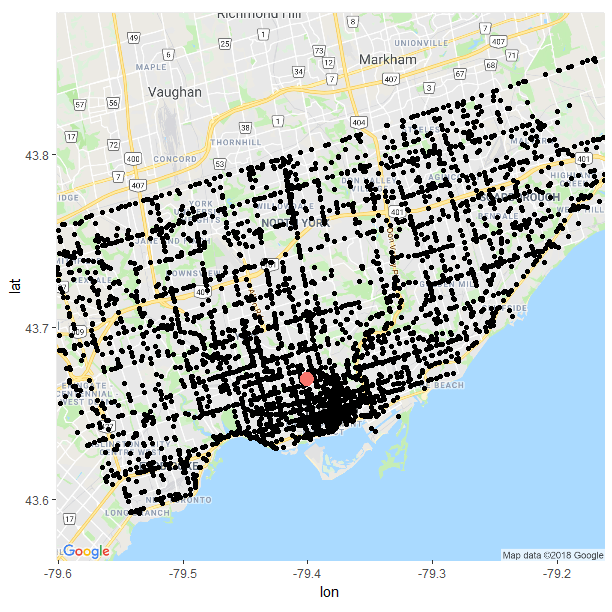
\includegraphics[scale=0.75]{WeatStat}
		\caption{The weather station (large red point) and observed collisions}
		\label{fig:weatherstation}
	\end{center}
\end{figure}

\begin{figure}[!h]
	\begin{center}
		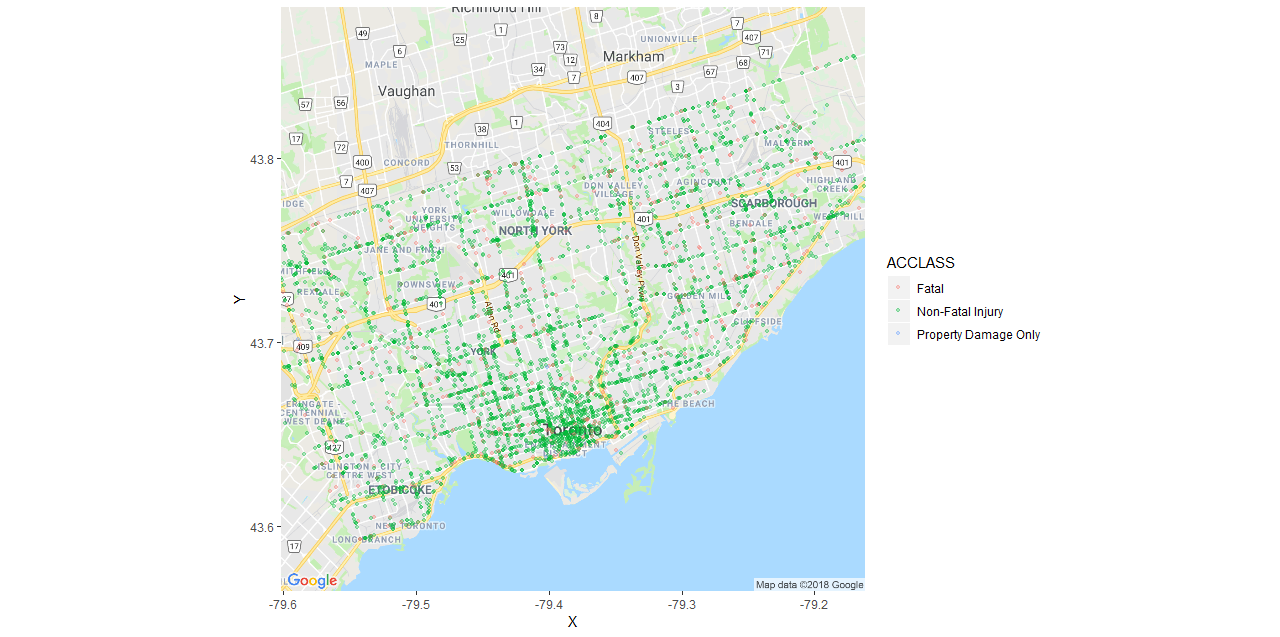
\includegraphics[scale = 0.5]{FatalityMap}
		\caption{Collisions coloured by severity of outcome}
		\label{fig:fatalitymap}
	\end{center}
\end{figure}

\begin{figure}[!h]
	\begin{center}
		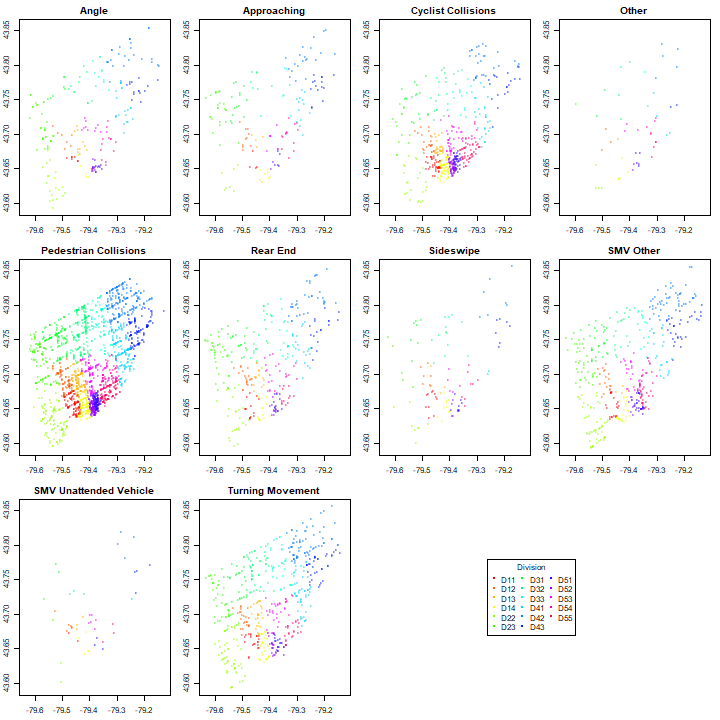
\includegraphics[scale = 0.75]{impactPanel}
		\caption{Collision locations, panelled by impact type, and coloured by the TPS division that responded}
		\label{fig:impactpanel}
	\end{center}
\end{figure}

\begin{figure}[!h]
	\begin{center}
		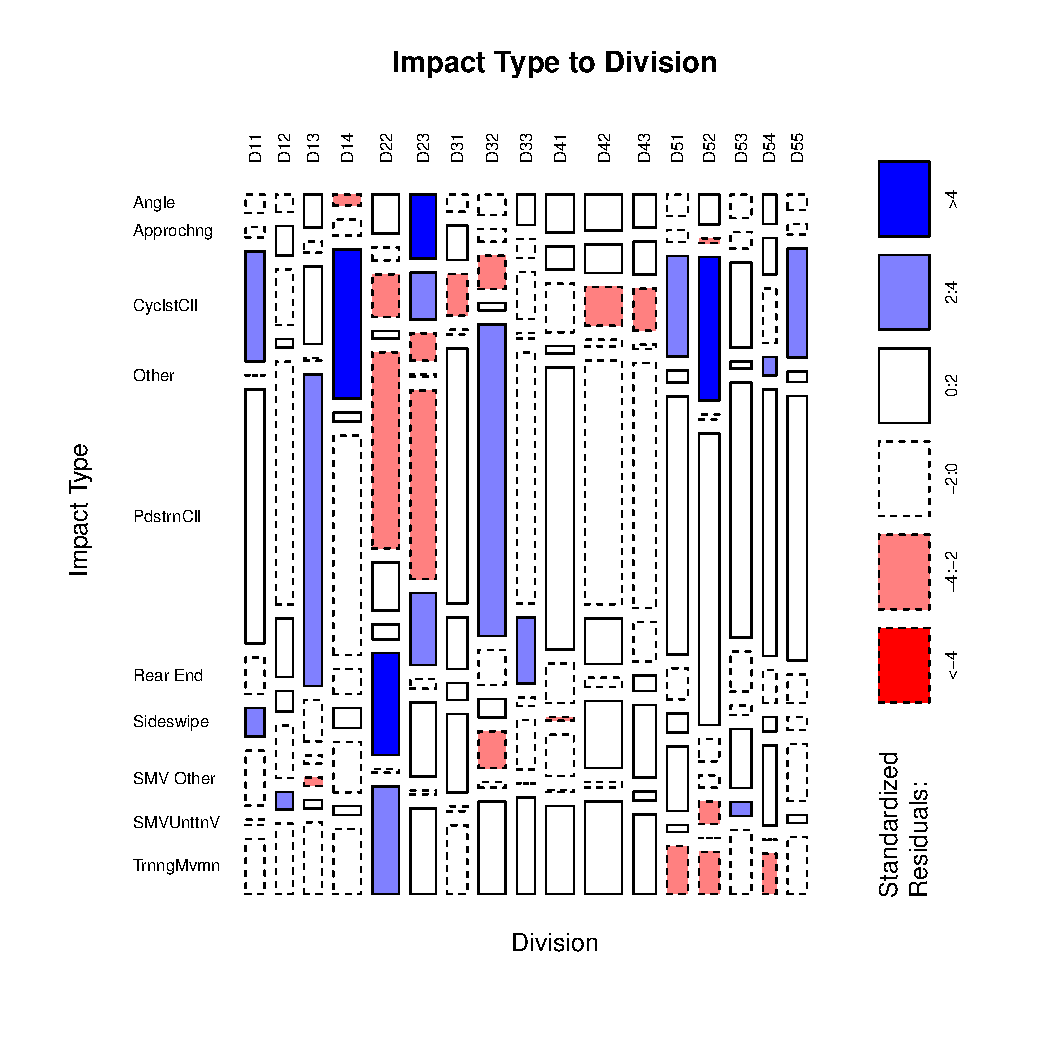
\includegraphics[scale = 1]{impactDivision}
		\caption{Impact type by TPS division responding, with statistically significant differences shaded}
		\label{fig:impactdivision}
	\end{center}
\end{figure}

\begin{figure}[!h]
	\begin{center}
		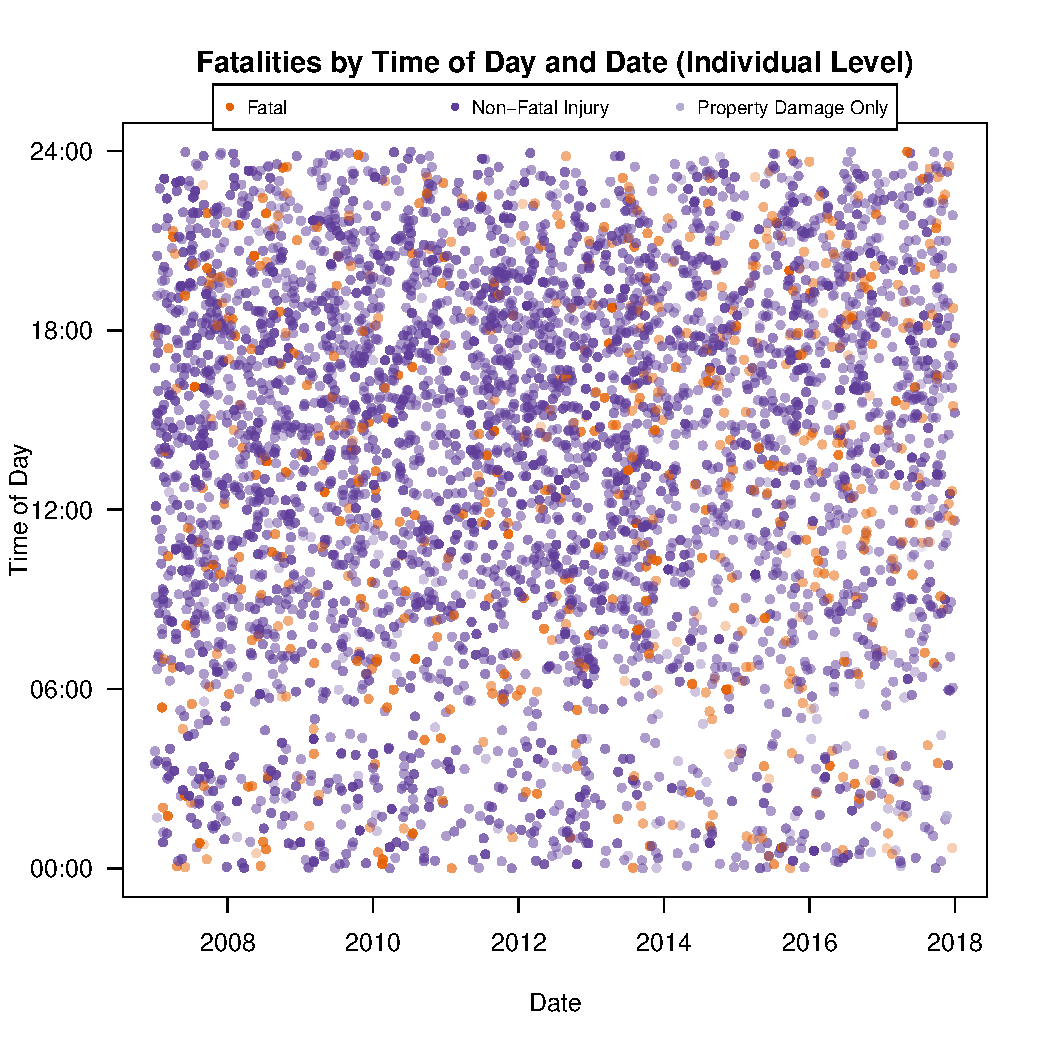
\includegraphics[scale = 1]{timedayind}
		\caption{Collision severity by time of day and date, displayed on the involved individual scale}
		\label{fig:timedayind}
	\end{center}
\end{figure}

\begin{figure}[!h]
	\begin{center}
		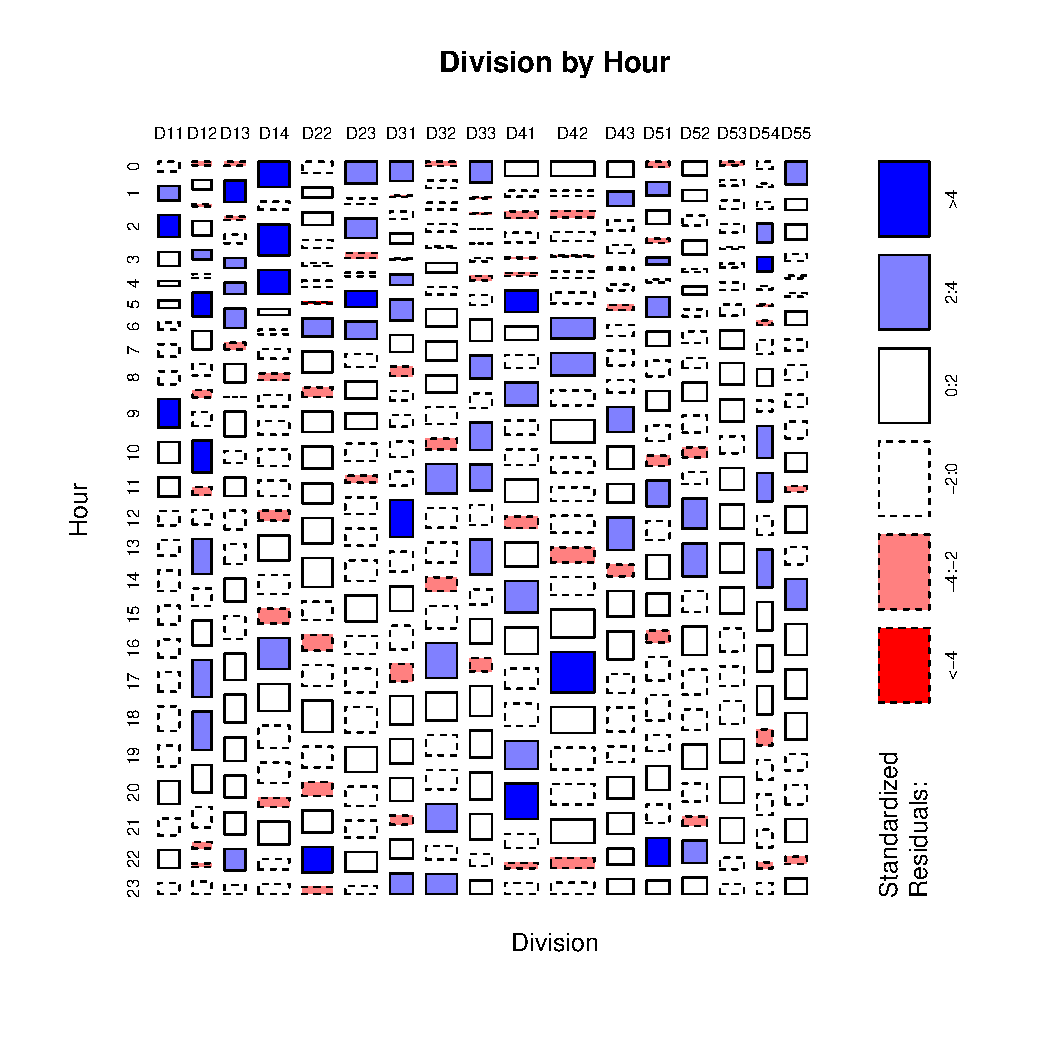
\includegraphics[scale = 1]{divisionhour}
		\caption{Mosaic plot of TPS division and hour, showing very different time profiles for each division}
		\label{fig:divisionhour}
	\end{center}
\end{figure}

\begin{figure}[!h]
	\begin{center}
		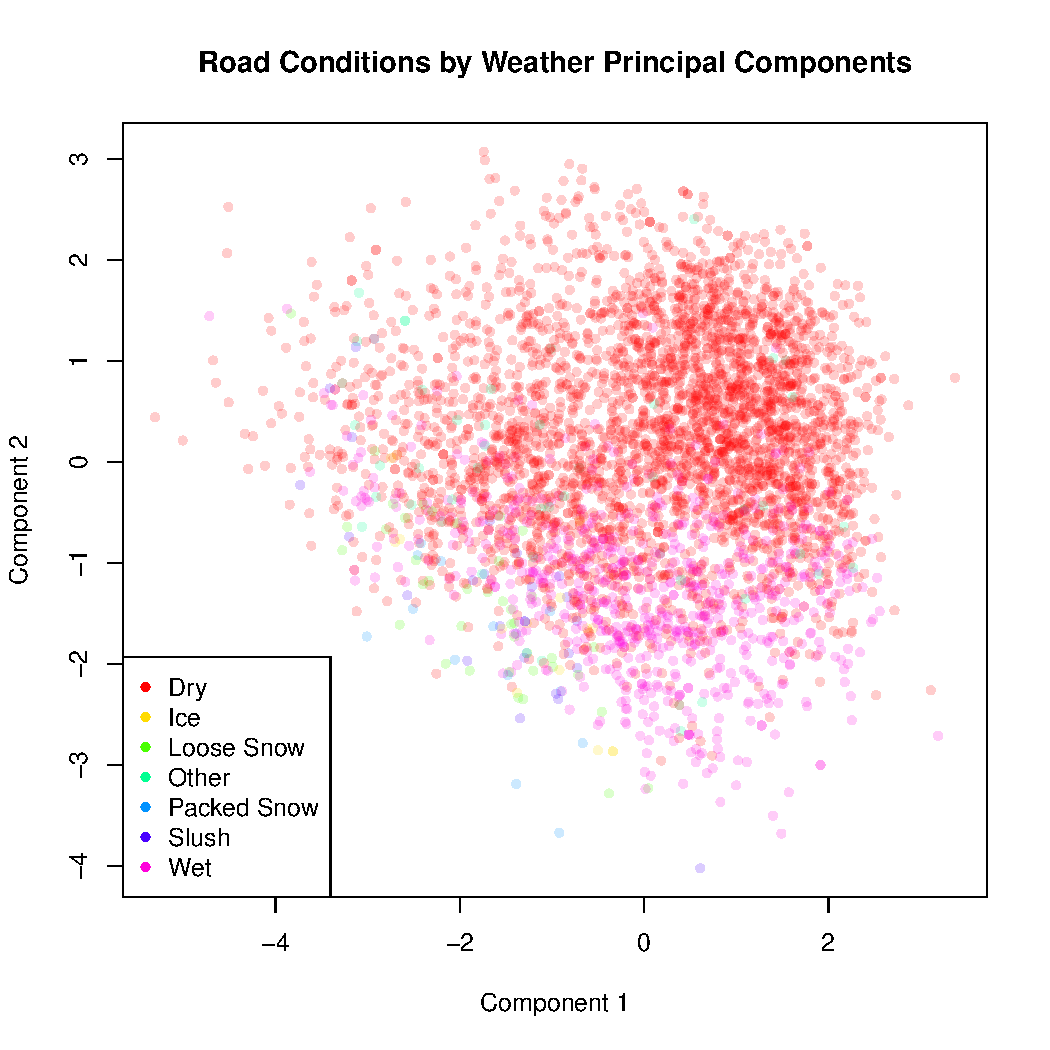
\includegraphics[scale = 1]{roadcondweather}
		\caption{Plot of weather principal components coloured by road conditions, note the separation of the different colours of points}
		\label{fig:roadcondweather}
	\end{center}
\end{figure}

\clearpage

\title{Code}
\begin{lstlisting}
##################################################

## TPS Data Scientist Application Project
## Christopher Salahub

##################################################

## Packages ######################################
library(MASS)
library(ggplot2)
library(ggmap)
library(stringr)
library(lme4)
library(lattice)


## Constants #####################################
## data locations
accidentData <- "KSI.csv"
## Canada weather stations
url.weather <- "ftp://ftp.tor.ec.gc.ca/Pub/Get_More_Data_Plus_de_donnees/Station%20Inventory%20EN.csv"
weatherstations <- "StationInventoryEN.csv"

## colour palette from colorbrewer
pal4 <- c("#e66101", "#fdb863", "#b2abd2", "#5e3c99")
pal3 <- pal4[c(1,4,3)]

## other palettes
pal.div <- rainbow(length(levels(ksi.accsimp$Division)))
pal.imp <- rainbow(length(levels(ksi.accsimp$IMPACTYPE)))

## map constants
TorontoMap <- get_map(location = c(left = min(ksi$X), right = max(ksi$X), top = max(ksi$Y), bottom = min(ksi$Y)),
                      maptype = "roadmap")
SimpleTo <- ggmap(TorontoMap)
Toronto <- ggmap(TorontoMap, base_layer = ggplot(aes(x = X, y = Y, color = ACCLASS), data = ksi.accsimp))


## Functions #####################################
## make UNIX day and hour helpers
UNIXday <- function(numdate) floor(as.numeric(numdate)/86400)
UNIXhour <- function(numdate) floor(as.numeric(numdate)/3600)

## small POSIX extraction helpers
hour <- function(numdate) as.numeric(format(numdate, "%H"))
minute <- function(numdate) as.numeric(format(numdate, "%M"))
day <- function(numdate) as.numeric(format(numdate, "%d"))
month <- function(numdate) as.numeric(format(numdate, "%m"))
year <- function(numdate) as.numeric(format(numdate, "%Y"))

## a helper to process the climate data pulled from the climate site
climatescan <- function(scanned) {
    ## first split everything by comma delimiter
    fielded <- str_split(scanned, pattern = ",")
    ## now remove the extraneous quotations
    quotecleaned <- lapply(fielded, str_replace_all, pattern = '\"', replacement = "")
    ## pad the results to account for missing entries
    quotecleaned <- lapply(quotecleaned,
                           function(el) {
                               if (length(el) != length(quotecleaned[[1]])) {
                                   c(el, rep("", length(quotecleaned[[1]]) - length(el)))
                               } else el
                           })
    ## create a data frame from the result
    colnames <- quotecleaned[[1]]
    data <- quotecleaned[2:length(quotecleaned)]
    scanned.frame <- as.data.frame(matrix(unlist(data), ncol = length(colnames),
                                          byrow = TRUE, dimnames = list(NULL, colnames)),
                                   stringsAsFactors = FALSE)
    ## now convert appropriate columns to numeric variables
    scanned.frame <- as.data.frame(lapply(names(scanned.frame),
                                          function(name) {
                                              if (grepl("Temp|Month|Year|Day|Hum|Visib|Press|Chill|Wind", name)) {
                                                  suppressWarnings(as.numeric(scanned.frame[,name]))
                                              } else scanned.frame[,name]
                                          }))
    names(scanned.frame) <- colnames
    return(scanned.frame)
}

## a functionto pull and process climate data tables
ClimatePull <- function(yearrng = NULL, region = "TORONTO", save = FALSE) {
    ## define the climate url components
    url.base <- "http://climate.weather.gc.ca/climate_data/bulk_data_e.html?format=csv&stationID="
    url.year <- "&Year="
    url.month <- "&Month="
    url.end <- "&Day=14&timeframe=1&submit= Download+Data"
    ## start setting region to capital letters for easier specification
    region <- toupper(region)
    ## now pull the station list and identify the stations (the url is restricted so this doesn't work, saved manually)
    ## stations <- read.table(url.weather, header = TRUE, skip = 3)
    stations <- read.csv(weatherstations, header = TRUE, skip = 3)
    ## get only the stations of interest
    names(stations) <- str_replace_all(names(stations), "[\\.]{1,}", "")
    stations <- stations[grepl(region, stations$Name),]
    ## compare the station data to the year range specified
    validstations <- with(stations, HLYFirstYear <= yearrng[1] & HLYLastYear >= yearrng[2])
    ## deal with situation of incomplete data by stopping function
    stopifnot(any(validstations))
    ## consider only valid stations
    stations <- stations[which(validstations),]
    ## for each extract data over the entire year range
    ## first specify some necessary extraction variables
    yearseq <- seq(yearrng[1], yearrng[2], by = 1)
    yearmonthspec <- cbind(rep(yearseq, each = 12),
                           rep(1:12, times = length(yearseq)))
    rownames(yearmonthspec) <- apply(yearmonthspec, 1, function(row) paste0("Y",row[1],"M",row[2]))
    ## now extract the data
    weatherdata <- lapply(stations$StationID,
                          function(stat) apply(yearmonthspec, 1,
                                                function(row) {
                                                    ## use the climate data url to pull data
                                                    yrmn <- row
                                                    scanned <- scan(paste0(url.base, stat, url.year, yrmn[1], url.month,
                                                                           yrmn[2], url.end),
                                                                    skip = 15, what = character(), sep = "\n")
                                                    ## use the earlier defined helper to process this scan
                                                    climatescan(scanned)
                                                }))
    weatherdata <- list(Key = stations, Data = weatherdata)
    ## now save this if desired
    if (save) {
        ## check directory existence
        if (!dir.exists("ClimateData")) {
            ## if it doesn't exist create it
            dir.create("ClimateData")
        }
        ## now save the data
        saveRDS(weatherdata, file = "ClimateData/weather.Rds")
    }
    ## return the result
    weatherdata
}

## write a function to restructure the data lists into one data frame
listRestructure <- function(list) {
    ## extract column names
    globNames <- names(list[[1]])
    ## generate data frame to hold all variables
    df <- data.frame(lapply(globNames, function(nm) unlist(lapply(list, function(el) el[,nm]))))
    names(df) <- globNames
    ## return this
    df
}

## create a panel plot function for easy spatial exploration
panelPlot <- function(data, panelling, ...) {
    ## get the number of levels
    levs <- levels(data[[panelling]])
    nlevs <- length(levs)
    ## near square root to create grid parameters
    nsq <- ceiling(sqrt(nlevs))
    nrws <- ceiling(nlevs/nsq)
    ## set parameters
    defpar <- par()
    par(mfrow = c(nrws, nsq), mar = defpar$mar/sqrt(nsq))
    ## create plots
    call <- match.call(expand.dots = FALSE)$`...`
    for (lev in levs) {
        with(data[data[[panelling]] == lev,], do.call(plot, as.list(call)))
    }
}

## Pre-Processing ################################
## start with some basic cleaning/variable synthesis
## load the data
ksi <- read.csv(accidentData)
ksi.pure <- read.csv(accidentData)
## clean it up a bit
names(ksi)[1] <- "X"
ksi$LATITUDE <-  NULL
ksi$LONGITUDE <- NULL
ksi$Index_ <- NULL
## remove the ID variables: all of their information is captured in the names
ksi$Hood_ID <- NULL
ksi$Ward_ID <- NULL
## clean up the road class variables
ksi$ROAD_CLASS <- as.factor(str_replace(str_replace(ksi$ROAD_CLASS, "Laneway", "Local"),
                                        " Ramp", ""))
## and the location coordinates
ksi$LOCCOORD <- as.factor(str_replace(ksi$LOCCOORD, "^ |Park, Private Property, Public Lane|Entrance Ramp Westbound",
                                      "Other"))
## and the visibility data
ksi$VISIBILITY <- as.factor(str_replace(str_replace(ksi$VISIBILITY, "^ |Strong wind", "Other"), "Drifting Snow",
                                        "Snow"))
## and the light data
ksi$LIGHT[ksi$LIGHT == " "] <- "Other"
ksi$LIGHT <- as.factor(as.character(ksi$LIGHT))
## and the surface condition data
ksi$RDSFCOND <- as.factor(str_replace(ksi$RDSFCOND, "Loose Sand or Gravel|Spilled liquid|^ ", "Other"))
## and the traffic control
ksi$TRAFFCTL <- as.factor(str_replace(ksi$TRAFFCTL, "^ |Police Control|School Guard|Streetcar \\(Stop for\\)|Traffic Gate|Yield Sign",
                                      "Other"))


## make the time variable more informative
ksi$PadTime <- sapply(ksi$TIME,
                           function(el) paste0(paste0(rep(0, times = 4 - nchar(el)), collapse = ""), el))
## there is no date/time variable, create one
ksi$Date <- substr(ksi$DATE, 0, 10)
ksi$DateTime <- as.POSIXct(x = paste(ksi$Date, ksi$PadTime, sep = " "),
                           tz = "EST", format = "%Y-%m-%d %H%M")
ksi$DATE <- NULL
## set the involvement variables to be indicators
ksi <- as.data.frame(lapply(ksi, function(var) if (identical(levels(var), c(" ", "Yes"))) as.numeric(var) == 2 else var))
## set the injury and age factors to be ordered
ksi$INJURY <- factor(as.character(ksi$INJURY), levels = c(" ", "None", "Minor", "Minimal", "Major", "Fatal"),
                     ordered = TRUE)
ksi$INVAGE <- factor(ksi$INVAGE, levels = c("unknown", "0 to 4", "5 to 9", levels(ksi$INVAGE)[-c(1,10,21)]), ordered = TRUE)

## extract the unique dates
length(ksi.unqDays <- sort(unique(as.POSIXct(ksi$Date, format = "%Y-%m-%d", tz = "EST"))))
## so we have 12557 individuals injured or killed over 2641 days, an average of roughly 5 per day
length(ksi.unqAcc <- unique(ksi$ACCNUM))
## the data covers 4400 reported accidents

## extract year range for climate data extraction
ksi.yearrange <- range(ksi$YEAR)
## get the weather data
if (file.exists("ClimateData/weather.Rds")) {
    climateData <- readRDS("ClimateData/weather.Rds")
} else climateData <- ClimatePull(yearrng = ksi.yearrange, save = TRUE)
## for our particular case there is only one relevant station
as.character(climateData$Key$Name)
plot(ksi$X, ksi$Y, pch = 20)
points(climateData$Key$LongitudeDecimalDegrees, climateData$Key$LatitudeDecimalDegrees, pch = 19,
       col = 'red')
points(mean(ksi$X), mean(ksi$Y), pch = 15, col = 'blue')
## thankfully it is not too far from the mean location of the points, in any case, extract the data from this list
climateData.data <- listRestructure(climateData$Data[[1]])
climateData.data$Time <- as.numeric(climateData.data$Time) - 1
climateData.data$DateTime <- as.POSIXct(climateData.data$`Date/Time`, format = "%Y-%m-%d %H:%M", tz = "EST")
## reformat column names to be more clear
names(climateData.data) <- str_replace_all(names(climateData.data), "\\(°C\\)|\\(.+\\)| ", "")
## remove uninformative columns
climateData.data <- climateData.data[,c("DateTime", "Year", "Month", "Day", "Time", "Temp",
                                        "DewPointTemp","RelHum","StnPress")]

## now add the weather data onto the KSI data
tempHour <- UNIXhour(climateData.data$DateTime)
ksi.weather <- sapply(UNIXhour(ksi$DateTime),
                      function(datetime) {
                          ## pull the correct row and data
                          reldata <- climateData.data[tempHour == datetime,
                                          c("Temp", "DewPointTemp", "RelHum", "StnPress")]
                          unlist(reldata)
                     })
ksi.weather <- data.frame(t(ksi.weather))

## perform a simple principal component analysis on the weather data to remove redundancy
weather.pca <- princomp(ksi.weather[apply(ksi.weather,1,function(row)!any(is.na(row))),], cor = TRUE)
summary(weather.pca)
## this suggests using the first two principal components for weather is likely adequate, as it accounts for
## most of the variation in the data
ksi.pcaweat <- as.matrix(scale(ksi.weather)) %*% weather.pca$loadings[,1:2]
colnames(ksi.pcaweat) <- paste0("Weather", colnames(ksi.pcaweat))
ksi.pcaweat <- as.data.frame(ksi.pcaweat)

## now combine with main dataset
ksi <- data.frame(ksi, ksi.weather, ksi.pcaweat)
## save if it is not already
if (!file.exists("KSI_weather.csv")) write.csv(ksi, "KSI_weather.csv", row.names = FALSE)

## create a new data set that resummarizes this by unique accidents, and by involved individual type
ksi.accidents <- aggregate(ksi, by = list(ksi$ACCNUM), FUN = unique)
ksi.accidents$Group.1 <- NULL
ksi.accidents$DateTime <- as.POSIXct(ksi.accidents$DateTime, tz = "EST")
## include a most severe injury factor, and oldest involved factor
ksi.accidents$WrstInj <- factor(as.character(sapply(ksi.accidents$INJURY, max)))
ksi.accidents$Oldest <- factor(sapply(ksi.accidents$INVAGE, max), levels = levels(ksi$INVAGE),
                               ordered = TRUE)
## include a variable for number of people involved
ksi.accidents$NumInv <- sapply(ksi.accidents$FID, length)
## now, as this accident summarized set is focused on the aspects causing accidents, remove items which cannot be summarized
## by uniqueness
ksi.accsimp <- ksi.accidents[,!sapply(ksi.accidents, is.list)]
## save both these objects
saveRDS(ksi.accidents, "KSI_accidents.Rds")
saveRDS(ksi.accsimp, "KSI_accidentssimplified.Rds")

## do a reverse operation, counting accidents in an hour window
tempHour <- UNIXhour(ksi.accidents$DateTime)
climateData.data$AccidentCount <- sapply(UNIXhour(climateData.data$DateTime),
                                         function(hour) sum(tempHour == hour))


## Investigation #################################
## start with some investigative plotting
## look spatially
plot(x = ksi.accsimp$X, y = ksi.accsimp$Y, pch = 20)
## try colouring by the division responding
with(ksi.accsimp, plot(x = X, y = Y, pch = 20, col = adjustcolor(pal.div[as.numeric(Division)], alpha.f = 0.2)))
## this is actually rather useful, we can see that the divisions are, for the most part, staying within their boundaries
## not super informative without a map, but there are some obvious patterns (i.e. streets appear quite clearly in this plot)
## colour by severity
with(ksi.accsimp, plot(x = X, y = Y, pch = 20, col = adjustcolor(pal3[as.numeric(ACCLASS)], alpha.f = 0.2)))
## colour by impact type
with(ksi.accsimp, plot(x = X, y = Y, pch = 20, col = adjustcolor(pal.imp[as.numeric(IMPACTYPE)], alpha.f = 0.2)))
## split by impact type to get even more detail
panelPlot(ksi.accsimp, "IMPACTYPE", x = X, y = Y, main = lev, pch = 20, xlim = range(ksi$X), ylim = range(ksi$Y),
          col = adjustcolor(pal.div[as.numeric(Division)], alpha.f = 0.3))
legend(x = "right", col = pal.div, legend = levels(ksi.accsimp$Division), xpd = NA, bg = "white", inset = -1.5, pch = 20,
       ncol = 3, title = "Division")
dev.off()
## add a map underneath
TorontoMap <- get_map(location = c(left = min(ksi$X), right = max(ksi$X), top = max(ksi$Y), bottom = min(ksi$Y)),
                        maptype = "roadmap")
Toronto <- ggmap(TorontoMap, base_layer = ggplot(aes(x = X, y = Y, color = ACCLASS), data = ksi.accsimp))
Toronto + geom_point(size = 1, alpha = 0.3)
## it seems there are no obvious spatial trends in the data

## now look at temporal variables
with(ksi.accsimp, plot(y = sort(YEAR), x = ppoints(length(YEAR))))
## relatively constant rates by year
with(ksi.accsimp, plot(y = sort(month(DateTime)), x = ppoints(length(DateTime))))
## relatively constant rates by month as well
with(ksi.accsimp, plot(y = sort(hour(DateTime)), x = ppoints(hour(DateTime))))
## very interesting, the accidents seem to occur mostly at night, with the hours between 5 and 10 looking safest,
## is there a difference depending on other variables?
with(ksi.accsimp, {
    plot(y = sort(hour(DateTime[WrstInj == "Fatal"])), x = ppoints(sum(WrstInj == "Fatal")))
    points(y = sort(hour(DateTime[WrstInj != "Fatal"])), x = ppoints(sum(WrstInj != "Fatal")),
           col = 'red')
})
## this suggests the time variable is more important for non-fatal accidents, which are further from uniformly
## distributed

## do some more simple time plotting, first by accident
with(ksi.accsimp, plot(x = DateTime, y = 60*hour(DateTime) + minute(DateTime), xlab = "Date", ylab = "Time of Day",
                       yaxt = 'n', pch = 20, col = adjustcolor(pal3[as.numeric(ACCLASS)], alpha.f = 0.3),
                       main = "Accident Fatalities by Time of Day and Date"))
axis(side = 2, at = c(0, 360, 720, 1080, 1440), labels = c("00:00", "06:00", "12:00", "18:00", "24:00"), las = 2)
legend(x = "top", legend = levels(ksi$ACCLASS), col = pal3, pch = 20, horiz = TRUE, xpd = NA, cex = 0.75,
       bg = "white", inset = -0.05)
## now for all individuals
with(ksi, plot(x = DateTime, y = 60*hour(DateTime) + minute(DateTime), xlab = "Date", ylab = "Time of Day",
                       yaxt = 'n', pch = 20, col = adjustcolor(pal3[as.numeric(ACCLASS)], alpha.f = 0.3),
                       main = "Accident Fatalities by Time of Day and Date"))
axis(side = 2, at = c(0, 360, 720, 1080, 1440), labels = c("00:00", "06:00", "12:00", "18:00", "24:00"), las = 2)
legend(x = "top", legend = levels(ksi$ACCLASS), col = pal3, pch = 20, horiz = TRUE, xpd = NA, cex = 0.75,
       bg = "white", inset = -0.05)
## those look very different, suggesting a relationship between time and number of individuals involved
with(ksi.accsimp, plot(x = 60*hour(DateTime) + minute(DateTime), y = NumInv, pch = 20,
                       col = adjustcolor(pal3[as.numeric(ACCLASS)], alpha.f = 0.2), xaxt = 'n',
                       xlab = "Time", ylab = "Number Involved in Accident"))
axis(side = 1, at = c(0, 360, 720, 1080, 1440), labels = c("00:00", "06:00", "12:00", "18:00", "24:00"))
ksi.accsimp$MininDay <- with(ksi.accsimp, 60*hour(DateTime) + minute(DateTime))
loess.numinv <- loess(NumInv ~ MininDay, data = ksi.accsimp)
lines(x = seq(0,1440,1), predict(loess.numinv, newdata = data.frame(MininDay = seq(0,1440,1))),
      col = 'black', lwd = 2)
## and here we can see that there is indeed a relationship, but it is perhaps weaker than expected
## maybe there is a spatial relationship?
scale.numInv <- max(ksi.accsimp$NumInv)
with(ksi.accsimp, plot(x = X, y = Y, pch = 20,
                       col = sapply(NumInv, function(n) rgb(n/scale.numInv,0,0,alpha=n/scale.numInv))))
mosaicplot(table(ksi.accsimp[,c("District", "NumInv")]))
mosaicplot(table(ksi.accsimp[,c("Ward_Name", "NumInv")]), shade = TRUE)
## if there is, it is weak
## maybe there is a relationship between division and number involved?
table(ksi.accsimp[,c("Division", "NumInv")])
mosaicplot(table(ksi.accsimp[,c("Division", "NumInv")]), shade = TRUE, ylab = "Number Involved",
           xlab = "Division", main = "Size of Accident by Division")
## also quite weak, but gives ideas

## perhaps the divisions deal with different kinds of accidents, look at fatalities by division
mosaicplot(table(ksi.accsimp[,c("Division", "ACCLASS")]), shade = TRUE, ylab = "Accident Class",
           main = "Accident Class by Division")
## once again, very homogeneous, it seems that divisions 32 and 41 handle slightly more fatal accidents than average and
## divisions 52 and 55 handle slightly fewer, but all must be prepared for any kind of accident
## try some more division relationships
mosaicplot(table(ksi.accsimp[,c("Division", "Hour")]), shade = TRUE)
## that's busy, try aggregating by four evenly-sized hour boundaries
hour.bound <- quantile(ksi.accsimp$MininDay, probs = seq(0,1,0.2))
tempbound <- 100*(hour.bound %/% 60) + hour.bound %% 60
hour.boundnames <- paste(tempbound[-6], tempbound[-1], sep = "-")
ksi.accsimp$AggTimes <- factor(hour.boundnames[sapply(ksi.accsimp$MininDay,
                                                      function(el) max(1,sum(hour.bound < el)))],
                               levels = hour.boundnames, ordered = TRUE)
mosaicplot(table(ksi.accsimp[,c("Division", "AggTimes")]), shade = TRUE)
## the aggregation changes the result slightly, but not too much
## check the division to impact type
mosaicplot(table(ksi.accsimp$Division,abbreviate(ksi.accsimp$IMPACTYPE, minlength = 9)), shade = TRUE, las = 2,
           xlab = "Division", ylab = "Impact Type")

## see if these aggregated times affect anything else
mosaicplot(table(ksi.accsimp[,c("ACCLASS", "AggTimes")]), shade = TRUE)
mosaicplot(table(ksi.accsimp[,c("ALCOHOL", "AggTimes")]), shade = TRUE) ## SUPER strong
with(ksi.accsimp, plot(x = DateTime, y = MininDay, pch = 20, main = "Alcohol and Time", ylab = "Time",
                       xlab = "Date", yaxt = "n",
                       col = adjustcolor(pal4[c(1,4)][ALCOHOL + 1], alpha.f = 0.2)))
axis(side = 2, at = c(0, 360, 720, 1080, 1440), labels = c("00:00", "06:00", "12:00", "18:00", "24:00"))
legend(x = "top", legend = c("Alcohol Not Involved", "Alcohol Involved"), col = pal4[c(1,4)], pch = 20, horiz = TRUE,
       xpd = NA, cex = 0.75, bg = "white", inset = -0.05)
mosaicplot(abbreviate(IMPACTYPE, minlength = 9) ~ AggTimes, data = ksi.accsimp, shade = TRUE, las = 2,
           main = "Impact Type by Time Windows", xlab = "Impact Type")
panelPlot(ksi.accsimp, "AggTimes", x = X, y = Y, main = lev, pch = 20,
          col = adjustcolor(pal4[c(1,4)][ALCOHOL + 1], alpha.f = 0.4))
legend(x = "right", legend = c("Alcohol Not Involved", "Alcohol Involved"), col = pal4[c(1,4)], pch = 20,
       xpd = NA, bg = "white", inset = -1)
dev.off()

## climate plots
with(ksi.accsimp, plot(x = Temp, y = StnPress, col = adjustcolor(pal3[as.numeric(ACCLASS)], alpha.f = 0.2), pch = 20))
with(ksi.accsimp, plot(x = WeatherComp.1, y = WeatherComp.2,
                       col = adjustcolor(pal3[as.numeric(ACCLASS)], alpha.f = 0.2), pch = 20))
## well, that is interesting, also no apparent relationship, maybe do some comparison with days without reports

## create distance matrix between points
ksi.dist <- dist(ksi.accsimp[,c("X","Y")])
## take the median as the reasonable bandwidth distance estimate
ksi.bandwidth <- median(ksi.dist)

## look at severity of accident by month
mosaicplot(table(data.frame(Month = as.factor(months(ksi.accsimp$DateTime)), WorstInjury = ksi.accsimp$WrstInj)), shade = TRUE,
           las = 2, main = "Severity to Month")
## now on the level of individuals
mosaicplot(table(data.frame(Month = as.factor(months(ksi$DateTime)), Severity = ksi$INJURY)), shade = TRUE,
           las = 2, main = "Severity to Month")
## these tell basically the same story, the month does not have a huge impact

## what about conditions
mosaicplot(table(ksi.accsimp[,c("WrstInj","RDSFCOND")]), las = 2)
## surprisingly no relationship observed
mosaicplot(table(ksi.accsimp[,c("NumInv","RDSFCOND")]), las = 2, shade = TRUE)
## once again, no serious relationship
mosaicplot(table(ksi.accsimp[,c("NumInv","VISIBILITY")]), las = 2, shade = TRUE)
## not alot there either
mosaicplot(table(ksi.accsimp[,c("WrstInj","VISIBILITY")]), las = 2, shade = TRUE)
## independent once again
mosaicplot(table(ksi.accsimp[,c("RDSFCOND","VISIBILITY")]), las = 2, shade = TRUE)
## strong relationship there (no surprise), they contain similar information

## look at sum by day for seasonality
tempdays <- UNIXday(ksi.accsimp$DateTime)
timespan <- seq(min(ksi.unqDays), max(ksi.unqDays), by = "day")
ksi.dayCounts <- sapply(UNIXday(timespan), function(el) sum(tempdays == el))
plot(x = timespan, y = ksi.dayCounts, type = 'l')
## too busy, try overplotting
tempyear <- year(timespan)
plot(NULL, xlim = c(1,366), ylim = range(ksi.dayCounts))
for (yr in unique(tempyear)) lines(1:sum(tempyear == yr), ksi.dayCounts[tempyear == yr])
## there is no detectable seasonality in the number of daily accidents

## try a simple glm on the climate data
climGLM <- glm(AccidentCount ~ as.factor(Month) + as.factor(Year) + as.factor(Time) + Temp + DewPointTemp +
             RelHum + StnPress, data = climateData.data, family = poisson)
## this matches the analysis performed above, we can see that the time being 4 am decreases the risk of severe
## accidents, and a slight positive relationship between temperature and negative for dew point, the air pressure
## does not seem to be significant

## try a more complicated model using mixed models to account for nested characteristics, here trying to predict
## accident occurrence based on information before the scene
## first: see if we can predict the serious injuries for involved persons
## first make a fatality indicator
ksi.accsimp$Fatality <- ksi.accsimp$WrstInj == "Fatal"
## select only model-relevant data
PredVars <- c("X","Y","YEAR","Hour","District","ROAD_CLASS","LOCCOORD","TRAFFCTL","VISIBILITY",
              "LIGHT","RDSFCOND","Ward_Name","WeatherComp.1","WeatherComp.2", "Fatality","Division")
ksi.predmod <- ksi.accsimp[,PredVars]
## add and do some clean up
ksi.predmod$YEAR <- as.factor(ksi.predmod$YEAR)
ksi.predmod$Hour <- as.factor(ksi.predmod$Hour)
ksi.predmod$Month <- as.factor(month(ksi.accsimp$DateTime))
## now try fitting the model based on weather, something available days in advance
mixedMod1 <- glmer(Fatality ~ ROAD_CLASS + VISIBILITY + RDSFCOND + WeatherComp.1 + WeatherComp.2 + (1 | Ward_Name) + (1 | Division),
                   data = ksi.predmod, family = binomial)
## this does not converge well, check variable relationships
with(ksi.predmod, plot(WeatherComp.1, WeatherComp.2, col = rainbow(length(levels(VISIBILITY)))[as.numeric(VISIBILITY)]))
with(ksi.predmod, plot(WeatherComp.1, WeatherComp.2, pch = 20, main = "Road Conditions by Weather Principal Components",
                       xlab = "Component 1", ylab = "Component 2",
                       col = adjustcolor(rainbow(length(levels(RDSFCOND)))[as.numeric(RDSFCOND)],alpha.f = 0.2)))
with(ksi.predmod, legend(x = "bottomleft", legend = levels(RDSFCOND), col = rainbow(length(levels(RDSFCOND))), pch = 20))
with(ksi.predmod, table(VISIBILITY, RDSFCOND))
## these results together demonstrate (at least part of) the problem, the road conditions, weather components, and visibility
## are highly related, for parsimony, stick with pca weather variables
mixedMod2 <- glmer(Fatality ~ Hour + ROAD_CLASS + WeatherComp.1 + WeatherComp.2 + (1|Ward_Name) + (1|Division),
                   data = ksi.predmod, family = binomial)
## still failed convergence, try removing hour
with(ksi.predmod, plot(WeatherComp.1, WeatherComp.2, col = rainbow(length(levels(Hour)))[as.numeric(Hour)]))
mixedMod3 <- glmer(Fatality ~ ROAD_CLASS + WeatherComp.1 + WeatherComp.2 + (1|Ward_Name) + (1|Division),
                   data = ksi.predmod, family = binomial)
## that worked, inspect results
dotplot(ranef(mixedMod3, which = "Ward_Name", condVar = TRUE), strip = FALSE)
dotplot(ranef(mixedMod3, which = "Division", condVar = TRUE), strip = FALSE)
## what about a model with hour instead?
mixedMod4 <- glmer(Fatality ~ Hour + WeatherComp.1 + WeatherComp.2 + (1|Ward_Name) + (1|Division),
                   data = ksi.predmod, family = binomial)
summary(mixedMod4)
summary(mixedMod3)
## comparing the AIC, model3 appears to be better
\end{lstlisting} \label{code}

\end{document}
